\outlineSubframe{Korrektheit eines Algorithmus}

\begin{frame}{Korrektheit von Algorithmen}{Allgemeines}
    \begin{itemize}[<+->]
        \item Jeder Algorithmus sollte auch in allen Fällen das korrekte Ergebnis liefern...
        \item Klingt simpel, aber eindeutiger Beweis für alle Eingaben oft schwierig
        \item Testen an ausgewählten Beispielen \textbf{nicht} ausreichend
        \begin{itemize}
            \item Jedoch verringern umfangreiche Tests natürlich das Risiko eines unentdeckten Fehler
        \end{itemize}
        \item Korrektheit lässt sich im Grunde nur durch formalen Beweis zeigen
        \begin{itemize}
            \item Wie zum Beispiel Induktionsbeweis
            \item Diese sind häufig sehr umfangreich und komplex...
            \item ...und deshalb auch nicht Teil der Vorlesung
        \end{itemize}
    \end{itemize}
\end{frame}

\begin{frame}{Korrektheit von Algorithmen}{}
\begin{minipage}{0.4\textwidth}
            \begin{figure}
                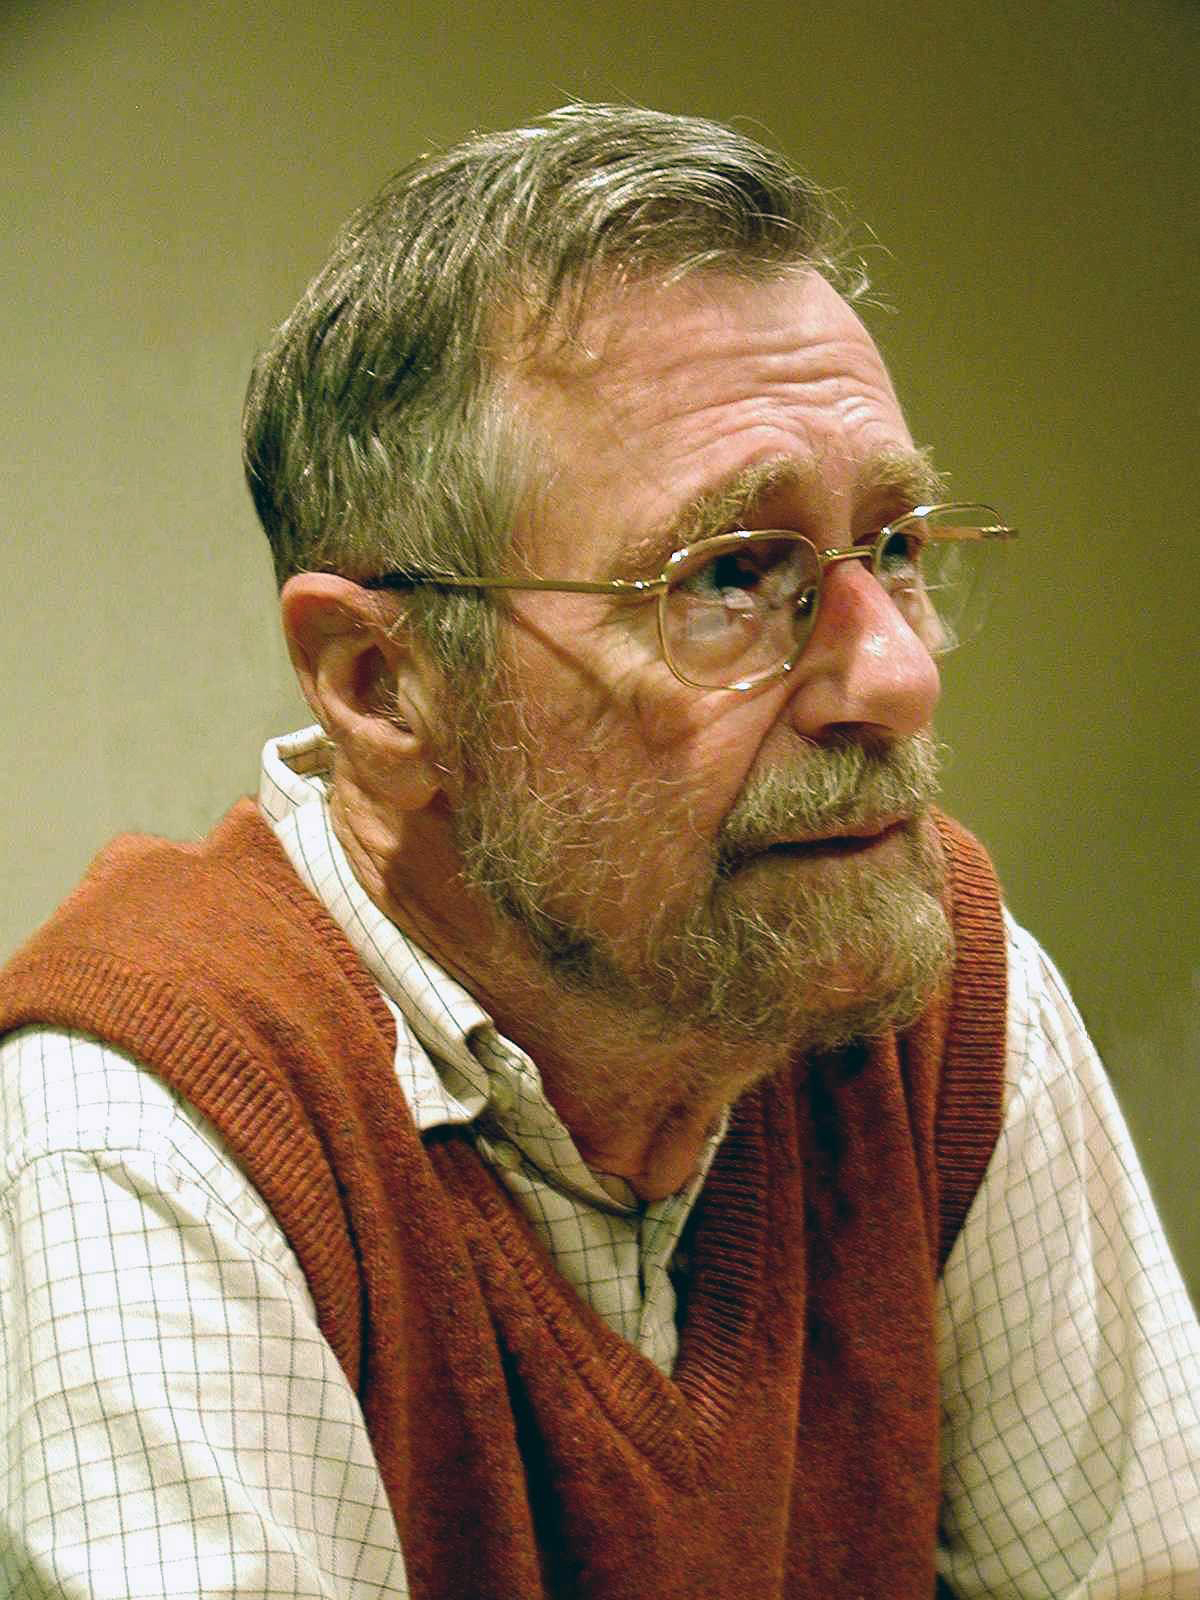
\includegraphics[height=4.5cm]{graph/dijkstra}
                \caption*{Quelle: }%\url{https://upload.wikimedia.org/wikipedia/commons/d/d9/Edsger_Wybe_Dijkstra.jpg}}
            \end{figure}
        \end{minipage}
        \hfill
        \begin{minipage}{0.55\textwidth}
            \textit{„Program testing can be used to show the presence of bugs, but never to show their absence!.“} \\\\Edsger W. Dijkstra
        \end{minipage}
\end{frame}

\outlineSubframe{Komplexitätsanalyse}

\begin{frame}{Speicherkomplexität}{Wie lässt sich diese messen?}
    \begin{itemize}[<+->]
        \item Wie schon erwähnt: Der verbrauchte Speicher ist Sprach- und Rechnerabhängig
        \item Mögliche Lösung über Definition von Referenzsprache und -system
        \item Messungen sind allerdings nicht repräsentativ
        \item Deswegen wird in der formalen Informatik mit dem \textit{Random-Access-Machine}(RAM) Modell gearbeitet
        \begin{itemize}
            \item Besteht im Grunde ausabzählbar unendlich vielen addressierbaren Speicherzellen
            \item Für einen Algorithmus wird dann bestimmt, wie viele Speicherzellen genutzt werden müssen
            \item Dies entspricht dann der Speicherkomplexität
        \end{itemize}
    \end{itemize}
\end{frame}

\begin{frame}{Laufzeitkomplexität}{Grundlegendes}
    \begin{itemize}[<+->]
        \item Gleiches Problem wie bei der Speicherkomplexität
        \item Deswegen hier ähnliches Modell:
        \begin{itemize}
            \item Man bestimmt die Anzahl von "`atomaren Operationen"' des Algorithmus
            \item Diese Operationen sind vergleichbar mit Assembler-Befehlsrepertoire
        \end{itemize}
        \item Beispiele für atomare Operationen:
        \begin{itemize}
            \item Addition/Subtraktion/Multiplikation/Division zweier Zahlen
            \item Lesen einer Variable von einer Speicheradresse
            \item Schreiben einer Variable an eine bestimmte Adresse
            \item Random Access in Arrays
            \item Vergleich zweier Zahlen
        \end{itemize}
    \end{itemize}
\end{frame}